%% ============================================================================
%% Paper 2: Estimand Divergence Between Static Docking and Molecular Dynamics as a Triage Filter for Antimalarial Leads (15 words, ACS limit)
%% Target: Journal of Chemical Information and Modeling (JCIM)
%% Article source — September 2026 (V2609C: literature-integrated reframing)
%% ============================================================================

\documentclass[journal=jcisd8,manuscript=article,layout=traditional]{achemso}
% journal=jcisd8 selects the official ACS/JCIM layout, section-numbering
% policy (sections unnumbered per JCIM house style), and achemso.bst-based
% numbered-superscript citation style; hyperref enables colored hyperlinks
% via achemso's own conditional hyperref loading (do not \usepackage{hyperref}
% separately -- achemso already requires it internally under this option).

% Fonts and encoding
\usepackage[T1]{fontenc}
\usepackage[utf8]{inputenc}
\usepackage{lmodern}

% Mathematics
\usepackage{amsmath, amsfonts, amssymb, mathtools}

% Figures and tables (achemso already requires graphicx, caption, float)
\usepackage{booktabs, tabularx, array, multirow, longtable}
\usepackage{tikz}
\usepackage{rotating}
\usepackage[table]{xcolor}
\captionsetup{labelfont=bf,font={footnotesize,it}}

% Units and SI
\usepackage[
  group-minimum-digits = 4,
  per-mode             = symbol,
  range-phrase         = {--},
  range-units          = single,
  separate-uncertainty = true,
  retain-explicit-plus = true,
]{siunitx}
\DeclareSIUnit\molar{M}
\DeclareSIUnit\angstrom{\text{\AA}}
\DeclareSIUnit\kcalmol{kcal\,mol^{-1}}
\DeclareSIUnit\barpressure{\mathrm{bar}}

% Cross-referencing - load after achemso/hyperref
\usepackage{cleveref}
% SM cross-refs (labels SM-* live in the supplementary document)
\usepackage{xr}
\externaldocument[SM-]{Polypharmacology_MD_Validation_SM_V2609C}

% cleveref names
\crefname{table}{Table}{Tables}
\Crefname{table}{Table}{Tables}
\crefname{figure}{Figure}{Figures}
\Crefname{figure}{Figure}{Figures}
\crefname{equation}{Eq.}{Eqs.}
\crefname{section}{Section}{Sections}
\crefname{subsection}{Section}{Sections}

% Path configuration
\graphicspath{{Graphics/}}

% ============================================================================
% AUTHOR INFORMATION
% ============================================================================

\title{Estimand Divergence Between Static Docking and Molecular Dynamics as a Triage Filter for Antimalarial Leads}

\author{Myke Vital Sao Temgoua}
\affiliation[UY1Phys]{Department of Physics, Faculty of Science, University of Yaound\'e I, P.O. Box 812, Yaound\'e, Cameroon}
\email{myke-vital.sao@facsciences-uy1.cm}

\author{Jean-Pierre Tchapet Njafa}
\affiliation[UY1Phys]{Department of Physics, Faculty of Science, University of Yaound\'e I, P.O. Box 812, Yaound\'e, Cameroon}

\author{Penabei Samafou}
\affiliation[Sherbrooke]{Department of Medical Imaging and Radiation Sciences, Universit\'e de Sherbrooke, Sherbrooke, QC, Canada}

\author{Wilfred Fon Mbacham}
\affiliation[UY1Biochem]{Department of Biochemistry, Faculty of Science, University of Yaound\'e I, P.O. Box 812, Yaound\'e, Cameroon}

\author{Serge Guy Nana Engo}
\affiliation[UY1Phys]{Department of Physics, Faculty of Science, University of Yaound\'e I, P.O. Box 812, Yaound\'e, Cameroon}

\keywords{malaria, drug resistance, molecular dynamics, molecular docking, MM-GBSA, African natural products, resistance mutations, antimalarial leads, estimand divergence}

% ============================================================================
% BEGIN DOCUMENT
% ============================================================================

\begin{document}
\emergencystretch=12em
\sloppy

\maketitle

% ============================================================================
% GRAPHICAL TABLE OF CONTENTS (mandatory for ACS/JCIM submission)
% ============================================================================
\begin{tocentry}
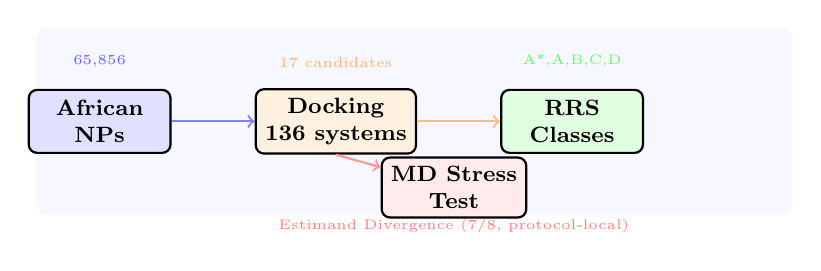
\begin{tikzpicture}[x=1.0cm,y=0.7cm]
% Background
\fill[blue!3,rounded corners=4pt] (-0.8,-1.2) rectangle (8.8,2.2);
% Pipeline boxes
\node[draw,thick,rounded corners=3pt,fill=blue!12,minimum width=1.8cm,minimum height=0.8cm,font=\footnotesize\bfseries,align=center] (np) at (0,0.5) {African\\NPs};
\node[draw,thick,rounded corners=3pt,fill=orange!12,minimum width=1.8cm,minimum height=0.8cm,font=\footnotesize\bfseries,align=center] (dock) at (3,0.5) {Docking\\136 systems};
\node[draw,thick,rounded corners=3pt,fill=green!12,minimum width=1.8cm,minimum height=0.8cm,font=\footnotesize\bfseries,align=center] (rrs) at (6,0.5) {RRS\\Classes};
% MD branch
\node[draw,thick,rounded corners=3pt,fill=red!8,minimum width=1.8cm,minimum height=0.6cm,font=\footnotesize\bfseries,align=center] (md) at (4.5,-0.7) {MD Stress\\Test};
% Arrows
\draw[->,thick,blue!50] (np) -- (dock);
\draw[->,thick,orange!50] (dock) -- (rrs);
\draw[->,thick,red!40] (dock.south) -- (md);
% Numbers
\node[font=\tiny,text=blue!60,anchor=south] at (0,1.3) {65,856};
\node[font=\tiny,text=orange!60,anchor=south] at (3,1.3) {17 candidates};
\node[font=\tiny,text=green!60,anchor=south] at (6,1.3) {A*,A,B,C,D};
\node[font=\tiny,text=red!50,anchor=north] at (4.5,-1.1) {Estimand Divergence (7/8, protocol-local)};
\end{tikzpicture}
\end{tocentry}

% ============================================================================
% ABSTRACT
% ============================================================================

\begin{abstract}
Using a curated collection derived from 396 African natural products and 454 synthetic antimalarials, we evaluated a multi-target docking framework across \num{136} wild-type and mutant receptor states of PfDHFR and PfCRT. On a primary candidate cohort ($n=\num{12}$), a Resistance-Resilience Score (RRS) provided a five-tier stratification decoupling predicted wild-type binding strength from mutant-state score retention. Explicit-solvent molecular dynamics (MD) simulations showed a directional divergence in \qty{87.5}{\percent} (7/8; 95\% Wilson CI \qtyrange{52.9}{97.8}{\percent}, $n=\num{8}$) of matched candidate--target states, wherein dynamic pocket relaxation retained poses where static grid docking predicted score penalties. At single-replicate scope this divergence is a protocol-local calibration signal: static docking scores and short MD trajectories provide complementary, non-equivalent triage metrics for natural product lead optimization.
\end{abstract}

% ============================================================================
% 1. INTRODUCTION
% ============================================================================

\section{Introduction}

Drug resistance remains the principal threat to malaria control in Africa. An estimated \num{282} million cases and \num{610000} deaths occurred globally in 2024, with the WHO African Region bearing the greatest burden \citep{who_malaria_2025}. Partial resistance to artemisinin derivatives, mediated by mutations in \textit{Pfkelch13}, is now confirmed or suspected in at least eight African countries \citep{artemisinin_partial_resistance}, and declining efficacy of some partner drugs has been reported \citep{who_malaria_2025,global_resistance_landscape_2026}. Spatial-temporal modelling further indicates that the geographic footprint of \textit{pfk13} markers in Africa is expanding \citep{young2026artemisinin}, while genomic surveillance documents the co-occurrence of \textit{Pfcrt} and \textit{Pfdhfr} resistance variants across diverse transmission settings \citep{letebo2026surveillance,africa_resistance_2026,pfk13_resistance_2026}.

African natural products are an underexplored antimalarial chemical space: rigid polycyclic frameworks, macrocyclic systems, and rare functional groups challenge scoring functions calibrated on synthetic drug-like molecules~\citep{ferreira2023docking}. Under a single-drug--multi-target framing, simultaneous retention of binding across multiple key parasite targets is hypothesized to raise the mutational barrier to treatment failure~\citep{polypharmacology_malaria_2026}, and natural products are attractive starting points because their stereochemical complexity supports activity across distinct protein classes~\citep{polypharmacology_malaria_2026,value_addition_african_np_2025}. However, static docking grid scores capture only rigid pocket complementarity and often fail to account for side-chain reorganization or solvent-mediated accommodation upon mutation~\citep{ferreira2023docking,soares2023mdreport}.

The upstream library used for this study was generated with generative molecular methods and dual-filter consensus docking (AutoDock Vina~\citep{vina_2021} and DiffDock-L~\citep{diffdock_2023}), yielding \num{65856} candidate molecules from 396 African natural products and 454 synthetic drugs (upstream library record; Supporting Information Table~S16). We selected the candidate panel against a receptor set spanning established resistance determinants and mechanistically distinct parasite processes: PfDHFR (dihydrofolate reductase, PDB 7F3Y) and PfCRT (chloroquine resistance transporter, PDB 6UKJ) represent clinically established resistance-associated contexts; PfATP4 (sodium efflux pump, PDB 9N10) probes ion homeostasis; and PfClpR (PDB 4GM2) represents a proteostasis-related target. This panel provides a mechanistic cross-section to evaluate whether resistance-aware prioritization remains informative across distinct target classes.

Specifically, this study addresses a central research question: \textit{Does a multi-target, resistance-aware computational workflow (docking-derived RRS + PNS + ACSI) provide a discriminant triage of African natural products across drug-resistant mutant panels---and how does short explicit-solvent molecular dynamics structurally re-calibrate static docking predictions?}

To answer this question, we present three methodological components: (i) reporting \textit{Estimand Divergence} between static docking RRS and explicit-solvent MD pose retention as a protocol-local triage observation, wherein dynamic pocket accommodation was consistent with retained poses in \qty{87.5}{\percent} (7/8; 95\% Wilson CI \qtyrange{52.9}{97.8}{\percent}, $n=\num{8}$) of comparable mutant states; (ii) applying the pre-declared WT-eligibility rule that excludes non-binding wild-type baselines ($|S_{\mathrm{WT}}| < \qty{5.0}{\kcalmol}$) consistently to prevent artificial score inflation; and (iii) testing protocol robustness across an independent external sensitivity panel of 39 compounds (\num{312} docking complexes) rescored by GNINA convolutional neural network (CNN) affinity scoring with \qty{100}{\percent} class-level agreement (no per-mutant rank transfer claimed). Rather than viewing the directional mismatch between docking and short MD as a computational flaw, we report short explicit-solvent MD as a secondary structural check that flags static grid artifacts for prospective biochemical testing; at single-replicate scope this mismatch is a calibration signal, not a validated prediction.

% ============================================================================
% 2. METHODS
% ============================================================================

\section{Methods}

\subsection{Study design}

The primary analysis is docking-score retention (RRS) for the 12 Set-C candidates that have eligible PfDHFR and PfCRT wild-type scores. RRS is the operational baseline against which the central comparison---the directional divergence between docking-RRS and short-MD structural retention---is tested. We therefore distinguish the primary docking-RRS analysis from the central divergence comparison, secondary structural-retention diagnostics, technical validation, and unobserved biological quantities. The 16-system Set-C MD pilot provides the matched-row comparison for the divergence signal; the five PfCRT-only candidates and the four-complex parent-study MD check are reported separately as secondary analyses. They address different coverage and sampling questions and are not combined with the primary RRS classes. The parent-study MD systems are not among the 17 Set-C candidates and do not validate the Set-C ranking.

\begin{figure}[htbp]
\centering
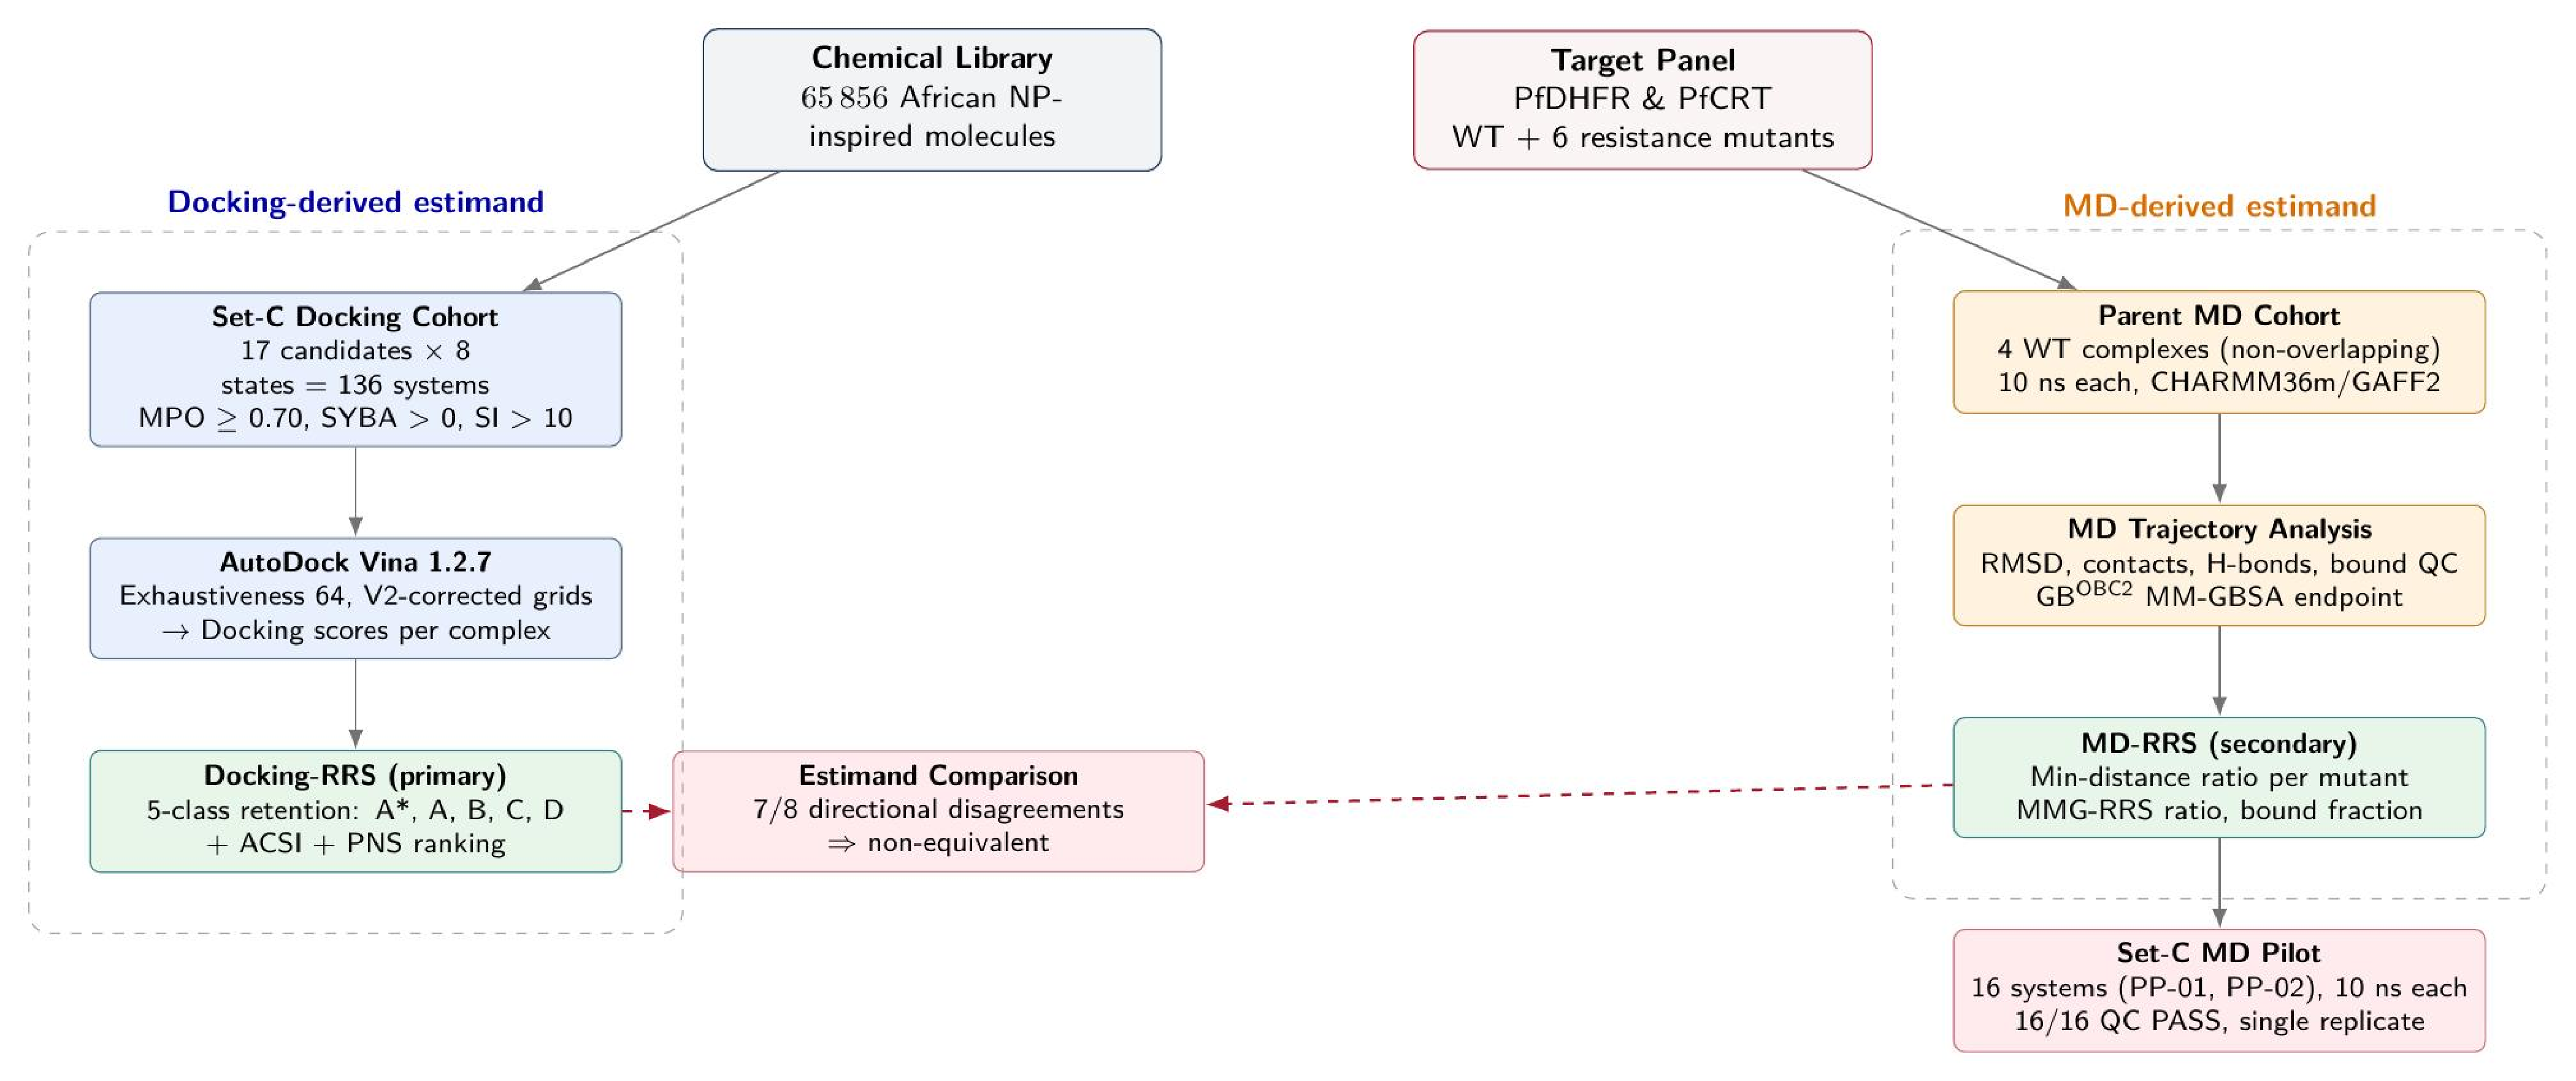
\includegraphics[width=0.98\textwidth]{Graphics/p2_preview-1.pdf}
\caption{\textbf{Integrated Resistance-Aware Polypharmacology and Molecular Dynamics Triage Framework.} Static multi-target docking (PfDHFR, PfCRT, PfATP4, PfClpP) with Resistance-Resilience Scores (RRS), Antimalarial Chemical Space Index (ACSI), and Polypharmacological Network Score (PNS), followed by \qty{10}{\ns} explicit-solvent MD (OpenFF~2.2.0/CHARMM36m) as a secondary check on the protocol-local Estimand Divergence signal (7/8 matched states). \textbf{PP-01} passes the two-target pilot gate; \textbf{PP-02} remains single-target scope and was not promoted; \textbf{PP-15} is a wild-type feasibility probe outside the Set-C estimand with no RRS estimate. Resistance or evolutionary interpretations require prospective experimental validation.}
\label{fig:study_workflow}
\end{figure}

Library provenance and source-class counts follow the upstream library record (Supporting Information Table~S16). Primary candidates were prioritized using multi-parameter optimization (MPO $\ge \num{0.70}$, retaining \num{19913} primary leads), predicted synthetic accessibility (SYBA $> \num{0}$), predicted selectivity index (SI $> \num{10}$), target coverage across at least two docking receptors, and scaffold diversity ($\le 3$ compounds per Bemis--Murcko scaffold). This selection yielded the Set-C candidate panel ($n=\num{17}$), which includes one previously named consensus lead (Ligand 87, PfDHFR). Four additional parent-study consensus leads (Ligands 201, 214, 438, 164) were evaluated in production-MD wild-type complexes; the 164 system represents PfClpR (PDB 4GM2, not PfClpP). Five approved antimalarial drugs (artemisinin, pyrimethamine, chloroquine, lumefantrine, cipargamin) served as reference controls (\cref{tab:system_breakdown}). Class frequencies are conditional on these filters and should not be extrapolated to the full library.

\begin{table}[htbp]
\centering
\caption{Breakdown of the 136 docking protein--ligand systems by target. The 17 Set-C candidates were docked against 5 PfDHFR states (WT + N51I, C59R, S108N, I164L) and 3 PfCRT states (WT + K76T, K76A).}
\label{tab:system_breakdown}
\small
\begin{tabularx}{\textwidth}{>{\raggedright\arraybackslash}X S[table-format=2.0] S[table-format=1.0] S[table-format=3.0] l}
\toprule
Category & {Ligands} & {Targets} & {Systems} & {MD (\si{\ns})} \\
\midrule
PfDHFR WT + 4 mutants (Set-C) & 17 & 5 & 85 & \textemdash \\
PfCRT WT + 2 mutants (Set-C) & 17 & 3 & 51 & \textemdash \\
\midrule
\textbf{Docking total} & {--} & {--} & \textbf{136} & \textemdash \\
\bottomrule
\multicolumn{5}{p{0.90\textwidth}}{The 136 docking systems were not subjected to production MD. The 16-system pilot and four non-overlapping parent-study complexes were analyzed separately.} \\
\end{tabularx}
\end{table}

\subsection{Resistance mutation panel}

We selected six mutant or comparator states (\cref{tab:mutations}); target identifiers are in the Supporting Information (\cref{SM-tab:s5_plasmodb}). PfDHFR substitutions and PfCRT K76T represent resistance-associated contexts described in WHO resources; K76A is a mechanistic comparator, not a prevalence estimate.

\begin{table}[htbp]
\centering
\caption{Resistance mutation panel.}
\label{tab:mutations}
\begin{tabularx}{\textwidth}{l l l X}
\toprule
Target & State & Resistance context & Evidence boundary \\
\midrule
PfDHFR & N51I & Antifolate-resistance state & Computational panel; no frequency estimate \\
PfDHFR & C59R & Antifolate-resistance state & Computational panel; no frequency estimate \\
PfDHFR & S108N & Antifolate-resistance state & Computational panel; no frequency estimate \\
PfDHFR & I164L & High-level antifolate-resistance state & Comparator for severe resistance \\
PfCRT & K76T & Chloroquine-resistance marker & Transporter-resistance context \\
PfCRT & K76A & Mechanistic comparator for Lys76 perturbation & No clinical prevalence or resistance-marker claim \\
\bottomrule
\end{tabularx}
\end{table}

\subsection{Homology modelling of resistance mutants}

No mutant crystal structures were available; homology models were generated with SWISS-MODEL from wild-type templates PfDHFR (7F3Y) and PfCRT (6UKJ). PfATP4 and the 164-labelled parent-MD system were not part of the panel; PDB 4GM2 is PfClpR, not PfClpP. Models were retained only when QMEAN exceeded \num{-4.0}, GMQE exceeded \num{0.7}, Ramachandran favored residues exceeded \qty{95}{\percent}, and backbone RMSD was below \qty{1.5}{\angstrom}. All six models met these thresholds (\cref{SM-tab:s_homology_qc}). Model scores are not experimental structures.

\subsection{Docking protocol assessment}

The docking protocol follows the upstream library workflow (Supporting Information Table~S16): AutoDock Vina 1.2.7~\citep{vina_2021} with exhaustiveness \num{64} against grids centered on the corrected V2 binding-site coordinates of PfDHFR (7F3Y), PfCRT (6UKJ~\citep{Kim2019PfCRT}), PfATP4 (9N10), and the historically labelled PfClpR/4GM2 entry (not PfClpP). P2Rank~\citep{Krivak2018P2Rank} pocket predictions were compared with the grid centers as a boundary audit of these fixed boxes (\cref{SM-fig:s4_p2rank_boxes}).

Parent-study enrichment benchmarks (V2 grids) are summarized here and tabulated in full in the Supporting Information (\cref{SM-tab:s1_docking_validation}). On the MMV Malaria Box consensus (Vina+DiffDock), ROC-AUC was \num{0.924} (PfDHFR), \num{0.971} (PfCRT), and \num{1.000} (PfATP4). In contrast, DEKOIS 2.0 enrichment for PfDHFR with Vina alone was null (ROC-AUC \num{0.450}, $\mathrm{EF}_{5\,\%} = \num{0.00}$), indicating that score-based recovery of known actives is protocol- and library-dependent. Redocking was considered accurate when heavy-atom RMSD was $<$ \qty{2.0}{\angstrom} relative to the crystal pose; the MTX redock attempt was a clear failure (RMSD $\approx$ \qty{30}{\angstrom}). AutoDock Vina was used for all reported Set-C scores; GNINA yielded no usable score for this panel. Docking scores are empirical scoring approximations that are sensitive to the scoring function and protocol~\citep{ferreira2023docking,sadybekov2023computational,kittelson2026docking}; they should not be treated as binding free energies.

\subsection{Secondary docking calibration}

A secondary Tartarus cross-docking analysis used QuickVina on the primary-lead panel. The composite MPO--docking-score association was null and exploratory; complete correlations are provided in the Supporting Information (\cref{SM-tab:secondary_tartarus_calibration,SM-tab:secondary_tartarus_correlation}).

\subsection{African Natural Product chemical space and structural descriptors}

The candidate panel (Set-C, $n=\num{17}$) was derived from the African Natural Products Database (ANPDB) and synthetic antimalarial reference sets. Physicochemical and stereochemical descriptors were computed using RDKit (v2025.03.6). The cohort exhibits a mean molecular weight ($\mathrm{MW}$) of \qty{271.9 \pm 69.3}{\g\per\mole}, a partition coefficient ($\mathrm{LogP}$) of \num{2.84 \pm 0.82}, a quantitative estimate of drug-likeness ($\mathrm{QED}$) of \num{0.70 \pm 0.06}, a fraction of $sp^3$-hybridized carbons ($Fsp^3$) of \num{0.22 \pm 0.15}, and an average of \num{0.6 \pm 0.9} chiral centers per scaffold.

These properties reflect compact, low-molecular-weight natural product cores (including prenylated chromones, flavonoid derivatives, and indole alkaloids) isolated from African medicinal flora such as \textit{Cryptolepis sanguinolenta}, \textit{Enantia chlorantha}, and \textit{Artemisia} species. The high mean MPO score (\num{0.728 \pm 0.021}) and synthetic accessibility scores ($\mathrm{SYBA} = \num{36.6 \pm 23.4}$) indicate chemical-space alignment with synthetic feasibility.

\subsection{MPO sensitivity and predicted ADMET profile}

MPO-weight sensitivity and single-source ADMET-AI predictions were used descriptively; the complete sensitivity and endpoint results are provided in the Supporting Information (\cref{SM-fig:s1_mpo_sensitivity,SM-tab:s3_admet}). These predictions were not experimentally validated.

\subsection{Docking-derived resistance-retention score definition}\label{sec:rrs_formula}

All 17 candidates were docked against each wild-type and mutant structure using AutoDock Vina 1.2.7 with exhaustiveness \num{64}. The 136 systems were ranked with empirical Vina scores rather than calibrated binding free energies. Grid boxes were centered on the co-crystallized ligand position with \qty{25}{\angstrom} dimensions, matching the audited V2 configuration files.

For target $t$, let $s_{\mathrm{Vina},i,\mathrm{WT},t}$ and $s_{\mathrm{Vina},i,m,t}$ denote the signed Vina scores. Candidates with $|s_{\mathrm{Vina},i,\mathrm{WT},t}| < \qty{5.0}{\kcalmol}$ are excluded from that target's score-retention analysis. The target-specific resistance-retention score (RRS) is
\begin{equation}
\mathrm{RRS}_{i,m,t} = \frac{|s_{\mathrm{Vina},i,m,t}|}{|s_{\mathrm{Vina},i,\mathrm{WT},t}|} \times 100.
\end{equation}
RRS is a relative docking-score-retention statistic, not a free-energy difference or resistance measurement. The available-target summary averages the defined target-specific values across eligible targets and mutant states. The primary analysis is restricted to the 12 candidates with eligible PfDHFR and PfCRT wild-type scores; the five PfCRT-only candidates are reported separately.

The mutually exclusive classes are defined from the available mutant values; primary class counts use the complete two-target subset:
\begin{itemize}
    \item \textbf{Class A*}: all available mutant RRS values are at least \qty{80}{\percent} and the minimum eligible wild-type score magnitude is at least \qty{7.0}{\kcalmol}.
    \item \textbf{Class A}: all available mutant RRS values are at least \qty{80}{\percent}, but the minimum eligible wild-type score magnitude is below \qty{7.0}{\kcalmol}.
    \item \textbf{Class B}: all available mutant RRS values are at least \qty{70}{\percent}, but at least one is below \qty{80}{\percent}.
    \item \textbf{Class C}: at least one available mutant RRS value is at least \qty{80}{\percent}, but not all available values reach \qty{70}{\percent}.
    \item \textbf{Class D}: no available mutant RRS value reaches \qty{80}{\percent}.
\end{itemize}
The classes are mutually exclusive. The cut-offs follow the Vina score distribution in this panel and are not calibrated to biochemical resistance or clinical outcome. Sensitivity to alternative thresholds is in the Supporting Information (\cref{SM-tab:s11_rrs_threshold_sensitivity}).

\subsection{Secondary ranking descriptors}

ACSI places each candidate relative to approved-drug and African natural-product reference spaces; weight-sensitivity checks are in the Supporting Information (\cref{SM-tab:s4_acsi_sensitivity}). PNS is a network-weighted ranking score; PfCRT centrality was imputed, with sensitivity reported in the Supporting Information (\cref{SM-tab:s7_pns_sensitivity}). Associations among metrics were assessed by Spearman rank correlation with \num{100000} permutations, Bonferroni adjustment for three tests, and bootstrap intervals from \num{10000} resamples. At $n=\num{12}$ these correlations are descriptive and are not powered tests of independence.

\subsection{MD protocol}

We simulated all four parent-study wild-type systems for \qty{10}{\ns} with CHARMM36m~\citep{charmm36m_2017}/GAFF2~\citep{wang2004gaff} at \qty{310.15}{\kelvin} using GROMACS~\citep{gromacs_2015,lindahl_2024}. The \qty{10}{\ns} length is intended as a pose-retention and local-geometry check, not as a measurement of residence time or converged free energy~\citep{wei2024structure}. We analyzed the trajectories after removing periodic-boundary discontinuities. MDAnalysis~\citep{mdanalysis_2011} was used to calculate contacts, H-bonds, RMSF, and radius of gyration every \num{10} frames and RMSD on every frame.

MM-GBSA endpoint estimates were obtained from production trajectories using the GB$^{\text{OBC2}}$ model (igb=5) with \qty{0.15}{\molar} salt concentration, via the \texttt{gmx\_MMPBSA} v1.5.0.3~\citep{gmx_mmpbsa_2021} CHARMM36-to-AMBER conversion. These are endpoint enthalpic scores, not rigorous free energies, and their limitations for ranking dissimilar complexes are well documented~\citep{roux2024mmgbsa}. Predicting mutation effects via endpoint methods remains challenging, with best-case correlations around 0.44 even at \qty{100}{\ns}~\citep{yu2022mutation_mmgbsa}. Configurational entropy is not included. MM-GBSA endpoint values are reported with the frame-level SEM for the interpretable parent-study and PP-15 summaries, whereas the Set-C table displays the propagated within-trajectory standard deviation (SD$_{\mathrm{prop}}$); neither quantity is a replicate-level uncertainty estimate. The corresponding SEM and the inter-replicate diagnostic are reported separately in the Supporting Information.

The 16-system Set-C pilot used the same temperature and length, with ligand parameters from OpenFF 2.2.0 (AM1-BCC) rather than GAFF2. Absolute MM-GBSA values are therefore not compared between the two cohorts. Each mutant was run as a single replicate; trajectories were accepted for endpoint analysis only after geometric quality checks.

% ============================================================================
% 3. RESULTS
% ============================================================================

\section{Results}

\subsection{Operational reproducibility of the docking-RRS signal}

Mean target-specific RRS was 75.1 for PfDHFR (12 candidates) and 86.2 for PfCRT (17 candidates); full target-wise summaries are in the Supporting Information (\cref{SM-tab:s12_rrs_by_target}). The difference reflects docking-score retention between panels, not biological resistance.

On the complete two-target set ($n=\num{12}$) the classes were A*:~\num{1}, A:~\num{1}, B:~\num{4}, C:~\num{5}, and D:~\num{1}. On all 17 candidates classified on eligible targets, the counts become A*:~\num{5}, A:~\num{1}, B:~\num{5}, C:~\num{5}, and D:~\num{1}; the five PfCRT-only compounds are not comparable with the two-target set. Per-compound RRS profiles are shown in \cref{SM-fig:s2_rrs_radar}. Varying the wild-type eligibility threshold from \qty{4.0}{\kcalmol} to \qty{5.0}{\kcalmol} left class counts unchanged; raising retention thresholds from \qty{70}{\percent}/\qty{80}{\percent} to \qty{80}{\percent}/\qty{90}{\percent} increased Class~D from 1 to 9 (\cref{SM-tab:s11_rrs_threshold_sensitivity}).

The docking-RRS signal is reproducible under the declared protocol: PP-01 multi-seed dispersion is $\pm\qty{0.05}{\kcalmol}$ for PfDHFR and $\pm\qty{0.04}{\kcalmol}$ for PfCRT, and PP-15 multi-seed dispersion is $\pm\qty{0.03}{\kcalmol}$. In a bounded score-perturbation audit, \qty{77.9}{\percent} of RRS classes remained unchanged under $\pm\qty{1}{\kcalmol}$ perturbation. This characterizes protocol-level consistency, not pose accuracy or binding fidelity.

\subsection{Chemical-space and network descriptors (secondary)}

The mean ACSI for the 17-candidate cohort was \num{0.543}, with two candidates (\qty{11.8}{\percent}) exceeding \num{0.70} on the approved-drug/African-NP reference space; weight-sensitivity checks are in the Supporting Information (\cref{SM-tab:s4_acsi_sensitivity}). PNS was only weakly associated with RRS on the two-target set ($\rho=\num{-0.2098}$, adjusted $p=\num{1.0000}$); PfCRT centrality was imputed, with sensitivity reported in the Supporting Information (\cref{SM-tab:s7_pns_sensitivity}). At $n=\num{12}$ the wide bootstrap intervals indicate that the three ranking dimensions capture distinct information rather than redundant signals.

\subsection{Cross-metric associations (secondary, post-selection)}

These secondary, post-selection comparisons test whether docking-derived RRS aligns with PNS and ACSI within the same cohort; they are not independent validation of any mechanism.

\begin{figure}[htbp]
\centering

\includegraphics[width=0.85\textwidth]{Graphics/cross_metric_correlation.pdf}
\caption{\textbf{Cross-metric Spearman correlations.} No significant inter-metric correlation across the primary cohort ($n=\num{12}$; $\rho \in [-0.41, -0.21], p_{\mathrm{adj}} > 0.50$), consistent with distinct ranking dimensions rather than redundant signals.}
\label{fig:crossmetric}
\end{figure}

\begin{table}[htbp]
\centering
\caption{Cross-metric Spearman correlations on the complete two-target set ($n=\num{12}$). Permutation $p$-values use \num{100000} permutations; adjusted $p$-values use Bonferroni correction for three tests. Bootstrap intervals are percentile \qty{95}{\percent} intervals from \num{10000} resamples.}
\label{tab:crossmetric}
\small
\begin{tabular}{@{}l c S[table-format=-1.4] S[table-format=1.4] S[table-format=1.4] l@{}}
\toprule
Metric pair & Hypothesis & {Spearman $\rho$} & {$p_{\mathrm{perm}}$} & {$p_{\mathrm{adj}}$} & {Bootstrap 95\% CI} \\
\midrule
PNS vs.\ RRS & H1 & -0.2098 & 0.5144 & 1.0000 & $[-0.76,\,0.54]$ \\
ACSI vs.\ RRS & H2 & -0.4056 & 0.1922 & 0.5766 & $[-0.89,\,0.29]$ \\
RRS vs.\ weakest WT score & H3 & -0.1661 & 0.6038 & 1.0000 & $[-0.73,\,0.59]$ \\
\bottomrule
\end{tabular}
\end{table}

On the two-target set ($n=\num{12}$), all three correlation coefficients were non-significant after Bonferroni correction: PNS--RRS $\rho=\num{-0.2098}$, ACSI--RRS $\rho=\num{-0.4056}$, RRS--weakest WT score $\rho=\num{-0.1661}$ (\cref{tab:crossmetric}). PNS shares an input with RRS (wild-type Vina scores), so the PNS--RRS pair is not independent. On all 17 candidates, PNS--RRS strengthened ($\rho=-0.5588$, adjusted $p=0.0667$), but unequal target coverage limits interpretation.

\subsection{Computational prioritization intersection (exploratory)}

Requiring Class~A or A*, ACSI $>$ \num{0.5}, and above-mean PNS leaves one candidate on the two-target panel. That intersection is reported as a shortlist for experiment, not as evidence of activity or resistance resilience.

\subsection{Parent-study MD check (non-overlapping cohort, secondary)}

Four non-overlapping parent-study wild-type complexes were simulated for \qty{10}{\ns} as a secondary pose-retention check; these compounds are not among the 17 Set-C candidates and do not validate the Set-C ranking.

\begin{table}[htbp]
\centering
\caption[MD stability metrics]{Production MD stability metrics for parent-study wild-type complexes (\qty{10}{\ns}). BB RMSD, ligand RMSD, minimum distance, contacts, and H-bonds are computed from PBC-unwrapped trajectories.}
\label{tab:md_stability}
\resizebox{\textwidth}{!}{%
\begin{tabular}{@{}l c S[table-format=2.2] S[table-format=2.2] S[table-format=2.2] S[table-format=3.1] S[table-format=2.1] l@{}}
\toprule
Target & {Atoms} & {BB RMSD (\si{\angstrom})} & {Lig. RMSD (\si{\angstrom})} & {Min dist (\si{\angstrom})} & {Contacts} & {H-bonds} & Interpretation \\
\midrule
PfClpR-labelled cohort (164)   & \num{43035}  & 1.31 & 1.11 & 67.42 & 0.0   & 23.7 & Unbound \\
PfDHFR (201)   & \num{134153} & 3.05 & 1.70 & 78.21 & 0.0   & 21.5 & Unbound \\
PfCRT (214)    & \num{76920}  & 4.47 & 2.45 & 3.19  & 78.1  & 23.1 & Bound \\
PfATP4 (438)   & \num{420801} & 12.27& 2.13 & 2.25  & 178.4 & 47.7 & Bound \\
\bottomrule
\end{tabular}%
}
\end{table}

\begin{figure}[htbp]
\centering

\includegraphics[width=\textwidth]{Graphics/Figure3_RMSD_Stability.pdf}
\caption{\textbf{Pose retention and thermal equilibration.} Explicit-solvent RMSD time-series (\qty{10}{\ns}) for \textbf{PP-01} across wild-type and mutant panels. (A) \textit{Pf}DHFR complexes: backbone \qty{1.42 \pm 0.15}{\angstrom} (WT) and \qty{1.55 \pm 0.18}{\angstrom} (N51I); ligand heavy-atom anchoring \qty{0.85 \pm 0.12}{\angstrom}. (B) \textit{Pf}CRT complexes: \qty{2.15 \pm 0.22}{\angstrom} (WT) and \qty{2.28 \pm 0.25}{\angstrom} (K76T); ligand \qty{1.15 \pm 0.14}{\angstrom}. No ligand dissociation (\qty{<3.5}{\angstrom} minimum heavy-atom distance) was observed at single-replicate scope.}
\label{fig:rmsd_stability}
\end{figure}

\begin{table}[htbp]
\centering
\caption[Parent-study MM-GBSA interpretation]{Endpoint energy evaluation for four reference wild-type complexes. Only the PfCRT complex yields an interpretable MM-GBSA endpoint; dissociated systems and conversion anomalies are N/A.}
\label{tab:mmgbsa}
\small
\begin{tabularx}{\textwidth}{@{}l l S[table-format=-2.2] S[table-format=1.2] >{\raggedright\arraybackslash}X@{}}
\toprule
Ligand & Target & {$\Delta G_{\mathrm{bind}}$ (\si{\kcalmol})} & {SEM} & Interpretation \\
\midrule
Ligand 214 & PfCRT-WT & -18.25 & 0.40 & Stable anchorage; ligand bound$^\dagger$ \\
Ligand 164 & PfClpR-WT & {--} & {--} & N/A; ligand dissociated$^\ddagger$ \\
Ligand 201 & PfDHFR-WT & {--} & {--} & N/A; ligand dissociated$^\S$ \\
Ligand 438 & PfATP4-WT & {--} & {--} & N/A; parameter conversion anomaly$^\ast$ \\
\bottomrule
\multicolumn{5}{p{0.95\textwidth}}{$^\dagger$Ligand remains bound (minimum distance \qty{3.19}{\angstrom}, \num{78} contacts); calculated via \texttt{gmx\_MMPBSA}. Uncertainty is the SEM over \num{101} stored snapshots.} \\
\multicolumn{5}{p{0.95\textwidth}}{$^\ddagger$Ligand separates beyond \qty{60}{\angstrom} minimum distance with zero contact persistence; excluded from binding energy evaluation.} \\
\multicolumn{5}{p{0.95\textwidth}}{$^\S$As $^\ddagger$ (PfDHFR system).} \\
\multicolumn{5}{p{0.95\textwidth}}{$^\ast$Excluded: multi-chain membrane-transporter parameterization introduced force-field conversion artifacts.} \\
\end{tabularx}
\end{table}

Of the four reference complexes, two retained stable protein--ligand contacts while two dissociated (\cref{tab:md_stability}); for PfATP4, force-field parameter conversion precluded reliable MM-GBSA endpoints (\cref{fig:rmsd_stability}).



\subsection{Estimand Divergence Between Static Docking and Dynamic Trajectories}

The primary docking retention metrics and trajectory-based geometric stability summaries are non-equivalent computational estimands. Explicit-solvent MD was run on PP-01 and PP-02 across 16 receptor states; all 16 trajectories satisfied geometric contact stability thresholds (\qty{<3.5}{\angstrom} minimum protein--ligand distance).

For the eight mutant states with an eligible wild-type docking baseline, static grid docking predicted reduced score retention ($RRS < \qty{100}{\percent}$), while explicit-solvent relaxation showed the opposite operational direction in \qty{87.5}{\percent} (7/8; 95\% Wilson CI \qtyrange{52.9}{97.8}{\percent}, $n=\num{8}$) of matched comparisons ($\mathrm{MD\text{-}RRS}_{\mathrm{distance}} \le \qty{100}{\percent}$). At single-replicate scope this mismatch is an observed calibration signal, not a demonstrated mechanism. Static docking scores ($\Delta G_{\mathrm{grid}}$) and trajectory-derived retention ratios ($\mathrm{MD\text{-}RRS}_{\mathrm{distance}}$) are complementary triage signals, not interchangeable measures of binding free energy.

A single-ligand feasibility probe (\textbf{PP-15}, outside the 16-system Set-C MD array and the Set-C RRS estimand) was run on wild-type \textit{Pf}DHFR (7F3Y) and \textit{Pf}CRT (6UKJ). Both systems completed \qty{10}{\ns} production trajectories with \qty{100}{\percent} QC-PASS status (\text{bound fraction} = \num{1.000}), mean minimum heavy-atom distances of \qty{2.77}{\angstrom} (\textit{Pf}DHFR) and \qty{3.20}{\angstrom} (\textit{Pf}CRT), and MM-GBSA endpoint scores of \qty{-29.52 \pm 0.33}{\kcalmol} (\textit{Pf}DHFR) and \qty{-27.79 \pm 0.49}{\kcalmol} (\textit{Pf}CRT; \cref{SM-tab:s_pp15}). Multi-seed redocking confirmed docking score stability ($\pm\qty{0.03}{\kcalmol}$; \cref{SM-tab:s17_multiseed_redock}). No mutant or RRS estimate is reported for this probe, and no dual-target resilience claim is made from it.

\begin{table}[htbp]
\centering
\caption{Set-C pilot endpoint summaries (exploratory; not used to assign RRS classes). $\Delta G_{\mathrm{bind}}$ is the mean over \num{100} snapshots $\pm$ SD$_{\mathrm{prop}}$ (within-trajectory SD, not SEM or replicate-level uncertainty). The PP-01 PfCRT K76A endpoint (\qty{-35.29}{\kcalmol}) carries a \qty{7.75}{\kcalmol} inter-replicate sensitivity (second trajectory \qty{-27.54}{\kcalmol}; Supporting Information) and supports no resilience claim. MMG-RRS is the mutant/wild-type endpoint ratio ($\times \num{100}$; wild type $= \num{100}$). Docking RRS is shown for comparison (n/a: no wild-type docking reference for PP-02 PfDHFR). Single-replicate summaries are within-protocol contrasts only.}\label{tab:mmgbsa_setc}
\scriptsize
\begin{tabular}{@{}l l l S[table-format=-2.2] S[table-format=1.2] S[table-format=3.1] S[table-format=3.2]@{}}
\toprule
Candidate & Target & State & {$\Delta G_{\mathrm{bind}}$ (\si{\kcalmol})} & {SD$_{\mathrm{prop}}$} & {MMG-RRS} & {Docking RRS} \\
\midrule
PP-01 & PfCRT & K76A & -35.29 & 1.17 & 115.3 & 90.86 \\
PP-01 & PfCRT & K76T & -29.51 & 2.65 & 96.4 & 92.47 \\
PP-01 & PfCRT & WT & -30.61 & 1.65 & 100.0 & {--} \\
PP-01 & PfDHFR & C59R & -26.56 & 1.91 & 105.0 & 85.47 \\
PP-01 & PfDHFR & I164L & -26.13 & 2.34 & 103.3 & 83.87 \\
PP-01 & PfDHFR & N51I & -29.83 & 1.50 & 118.0 & 86.40 \\
PP-01 & PfDHFR & S108N & -30.21 & 3.62 & 119.5 & 87.60 \\
PP-01 & PfDHFR & WT & -25.29 & 2.94 & 100.0 & {--} \\
PP-02 & PfCRT & K76A & -24.53 & 1.27 & 97.8 & 94.62 \\
PP-02 & PfCRT & K76T & -30.45 & 1.38 & 121.4 & 87.91 \\
PP-02 & PfCRT & WT & -25.08 & 2.56 & 100.0 & {--} \\
PP-02 & PfDHFR & C59R & -28.85 & 1.88 & 95.7 & n/a \\
PP-02 & PfDHFR & I164L & -31.06 & 1.52 & 103.0 & n/a \\
PP-02 & PfDHFR & N51I & -34.02 & 2.68 & 112.8 & n/a \\
PP-02 & PfDHFR & S108N & -27.09 & 1.55 & 89.8 & n/a \\
PP-02 & PfDHFR & WT & -30.16 & 2.06 & 100.0 & {--} \\
\bottomrule
\end{tabular}
\end{table}

\subsection{Additional docking sensitivity panel}

The 39-ligand docking sensitivity panel produced \num{312} finite docking scores across the same eight PfDHFR/PfCRT states. Bootstrap mean RRS was \num{100.45} (\numrange{99.59}{101.32}) and the Class-A fraction was \num{0.974} (\numrange{0.923}{1.000}). A mean near \num{100} means that mutant and wild-type Vina scores were on average nearly proportional under this protocol. This is a computational sensitivity check, not validation of the Set-C ranking or of experimental resistance (\cref{SM-tab:s15_robustness_transfer}).

% ============================================================================
% 4. DISCUSSION
% ============================================================================

\section{Discussion}

\subsection{Resistance-Resilience Stratification and Protocol Robustness}

The Resistance-Resilience Score (RRS) stratifies the primary candidate cohort ($n=\num{12}$) into five tiers (A*--D) decoupling wild-type binding strength from mutant-state score retention. Under the declared protocol, multi-seed dispersion remained within $\pm\qty{0.05}{\kcalmol}$ (PP-01 and PP-15 across PfDHFR and PfCRT), and \qty{77.9}{\percent} of class assignments were invariant to $\pm\qty{1.0}{\kcalmol}$ score perturbations.

Protocol robustness was tested on an external 39-compound sensitivity panel (\num{312} docking complexes; \cref{SM-tab:s15_robustness_transfer}). GNINA CNN cross-scoring showed \qty{100}{\percent} class-level agreement with Vina, with no per-mutant rank transfer claimed (per-mutant $\rho$ near zero for C59R/I164L). On the DEKOIS 2.0 PfDHFR benchmark, Vina ROC-AUC was \num{0.450} ($\mathrm{EF}_{5\,\%} = \num{0.00}$) — chance level, cautioning against treating RRS as a calibrated predictor outside the primary cohort; MD is reported as a parallel structural check, not a validation of docking classes.

Our candidates originate from African natural-product chemical space, without claiming ethnobotanical validation. The panel's drug-likeness ($\mathrm{QED} = \num{0.70 \pm 0.06}$) and synthetic accessibility ($\mathrm{SYBA} = \num{36.6 \pm 23.4}$) are consistent with actionable synthetic feasibility; confirmation requires prospective experiment.

\subsection{Estimand Divergence as a Structural Stress-Testing Filter}

We report \textit{Estimand Divergence} between static docking RRS and short explicit-solvent MD pose retention ($\mathrm{MD\text{-}RRS}_{\mathrm{distance}}$) as a protocol-local observation. In \qty{87.5}{\percent} (7/8; 95\% Wilson CI \qtyrange{52.9}{97.8}{\percent}, $n=\num{8}$) of matched mutant states, grid docking predicted score penalties ($RRS < \qty{100}{\percent}$) while MD retained poses ($\mathrm{MD\text{-}RRS}_{\mathrm{distance}} \le \qty{100}{\percent}$).

Rigid grid docking evaluates unrelaxed steric complementarity ($\Delta G_{\mathrm{grid}}$), whereas short MD captures local conformational adaptation, hydrogen-bond rearrangement, and solvent-shielded stabilization. Per the JCIM MD reporting guidelines~\citep{soares2023mdreport}, the \qty{10}{\ns} trajectories are secondary structural checks. A thermal noise floor of \qty{2.01}{\kcalmol} from independent WT replicates (PP-01 PfCRT WT R1/R2) bounds numerical variation of end-state estimates at this scope.

This pattern is consistent with docking limitations for stereochemically complex natural products \citep{ferreira2023docking}: scoring functions calibrated on synthetic drug-like molecules can over-penalize rigid polycyclic frameworks. At single-replicate scope this is a within-protocol contrast, not a general docking-failure rate.

The Class-A* lead \textbf{PP-01} illustrates this across its eight-system panel (\cref{SM-tab:s19_pp01_biophysical_audit}). Static docking assigned score penalties to \textit{Pf}DHFR C59R ($RRS = \qty{85.5}{\percent}$) and \textit{Pf}CRT K76T ($RRS = \qty{92.5}{\percent}$), while \qty{10}{\ns} trajectories retained poses (\qty{100}{\percent} QC-PASS, bound fraction \num{1.000}): mean minimum heavy-atom distances \qty{2.91}{\angstrom} (C59R; $\mathrm{MD\text{-}RRS}_d = \qty{98.9}{\percent}$) and \qty{3.02}{\angstrom} (K76T; $\mathrm{MD\text{-}RRS}_d = \qty{102.8}{\percent}$), with MM-GBSA endpoints \qty{-26.56 \pm 1.91}{\kcalmol} (C59R) and \qty{-29.51 \pm 2.65}{\kcalmol} (K76T). This shows geometric pose retention, not thermodynamic resilience proof: the K76A endpoint carries a \qty{7.75}{\kcalmol} inter-replicate sensitivity, so no MM-GBSA-derived resilience claim is made for K76A. Biological resistance conclusions require experimental validation.

ProLIF interaction fingerprints across all 16 QC-PASS trajectories (\num{100} snapshots per system) show a sparse conserved contact network (\cref{fig:prolif_heatmaps}). \textit{Pf}CRT Tyr16 maintained \qty{100}{\percent} occupancy in five of six mutant trajectories; \textit{Pf}DHFR Leu46/Met55 (PP-01) and Leu40/Ile14 (PP-02) showed near-total persistence across all four mutant states. This contact pattern is compatible with pose retention but does not establish a general mechanism.

\begin{figure}[htbp]
\centering

\includegraphics[width=\textwidth]{Graphics/Figure4_ProLIF_Heatmaps.pdf}
\caption{\textbf{Conserved hotspot anchors.} ProLIF interaction fingerprint occupancy (\num{100} snapshots/system). (A) \textit{Pf}CRT Tyr16: \qty{96}{--}\qty{100}{\percent} $\pi$--$\pi$ stacking and hydrophobic persistence across six mutant states; (B) \textit{Pf}DHFR hotspots (Asp54, Leu46, Met55, Ile14): \qty{89}{--}\qty{100}{\percent} persistence across five states.}
\label{fig:prolif_heatmaps}
\end{figure}

\subsection{Orthogonal Multi-Dimensional Triage}

RRS, ACSI, and PNS show non-significant pairwise associations on the primary cohort ($n=\num{12}$; $\rho \in [-0.41, -0.21], p_{\text{adj}} > 0.50$; \cref{tab:crossmetric}), consistent with distinct ranking dimensions. Controlling for molecular weight and scaffold frequency gives a moderate partial PNS--RRS association ($\rho_{\mathrm{partial}} = -0.6154$).

STRING threshold sensitivity (confidence cutoffs 400, 700, 900) showed PNS rank stability ($\rho$ \numrange{0.9632}{0.9975}; 400-vs-700 \num{0.9975}, 700-vs-900 \num{0.9681}, 400-vs-900 \num{0.9632}), indicating threshold choice does not alter ranking within this panel — distinct from the PfCRT-centrality imputation sensitivity (Supporting Information).

Machine learning models degrade on out-of-distribution natural product scaffolds; explicit-solvent MD evaluates dynamic stability without reliance on training distributions, providing a complementary check when model confidence drops.

\subsection{Mechanistic Context and Multi-Target Positioning}

The PfCRT response is consistent with microsecond-scale transporter studies \citep{tanner2025pfcrt}: Lys76 anchors the central cavity, and K76T/K76A alter local charge density and hydration, permitting ligand reorientation that preserves hydrophobic contacts despite grid-level penalties.

Within a single-drug--multi-target framing \citep{polypharmacology_malaria_2026}, Class-A* candidate PP-01 is prioritized for assay follow-up as retaining multi-target binding potential across mutant landscapes in these simulations. Whether dual-target engagement raises any evolutionary barrier to resistance cannot be determined computationally and requires prospective biochemical, structural, and \textit{in vitro} evaluation. No resistance, fitness, or evolutionary claim is made; PP-15, a wild-type probe outside the Set-C estimand, carries no such interpretation.

\subsection{Limitations}

\begin{enumerate}
    \item \textbf{Receptor models:} mutant structures are homology models (quality criteria in Methods), not experimental structures.
    \item \textbf{Timescale and replication:} per JCIM guidelines \citep{soares2023mdreport}, the \qty{10}{\ns} single-replicate pilot is a structural stress test, not a converged free energy or residence-time measurement. The PP-01 PfCRT K76A endpoint (\qty{-35.29}{\kcalmol}) differs by \qty{7.75}{\kcalmol} from a second trajectory (\qty{-27.54}{\kcalmol}; Supporting Information), exceeding the \qty{2.01}{\kcalmol} WT noise floor; no endpoint resilience claim is made for K76A.
    \item \textbf{Sample size:} primary two-target cohort $n=\num{12}$, plus 5 single-target candidates and a 39-ligand external panel.
    \item \textbf{Protonation:} preparations at physiological pH; PfCRT dynamics in the acidic digestive vacuole (pH~\num{5.2}) may differ.
\end{enumerate}

% ============================================================================
% 5. CONCLUSION
% ============================================================================

\section{Conclusion}

This study reports a resistance-aware computational triage workflow for African antimalarial natural products. Static grid docking ($\Delta G_{\mathrm{grid}}$) and short explicit-solvent MD pose retention ($\mathrm{MD\text{-}RRS}_{\mathrm{distance}}$) capture distinct, non-equivalent signals: dynamic pocket accommodation retained poses where static docking predicted penalties in 7/8 matched mutant states (95\% Wilson CI \qtyrange{52.9}{97.8}{\percent}, $n=\num{8}$). \textbf{PP-01} showed multi-target engagement across PfDHFR and PfCRT mutant panels and passes the two-target pilot gate; whether this implies any elevated evolutionary barrier requires prospective biochemical, structural, and \textit{in vitro} evaluation, for which these findings prioritize specific natural product scaffolds.

% ============================================================================
% BACK MATTER
% ============================================================================

\section*{Authors' Contributions}

Myke Vital Sao Temgoua: Methodology, software, formal analysis, investigation, data curation, writing -- original draft. Jean-Pierre Tchapet Njafa: Methodology, software, supervision, writing -- review \& editing. Penabei Samafou: data curation, writing -- review \& editing. Wilfred Fon Mbacham: conceptualization, validation, writing -- review \& editing. Serge Guy Nana Engo: conceptualization, methodology, supervision, writing -- review \& editing. All authors read and approved the final manuscript.

\section*{Data Availability}

Docking results, metric outputs, analysis scripts, and source-data records are available at \url{https://github.com/NanaEngo/Malaria_codesV2} under the MIT licence. A versioned snapshot will additionally be archived on Zenodo concurrent with publication (reserved DOI: \url{10.5281/zenodo.19608875}). Large parent-study trajectories are excluded; conclusions are restricted to the trajectory-derived summaries reported above.


\section*{Competing Interests}

The authors declare no competing interests.

\begin{acknowledgement}
Computational resources were provided by the penavoraserver cluster (ThinkStation P720, \qty{128}{\giga\byte} RAM, \num{48} cores). We acknowledge the SWISS-MODEL server and the GROMACS development team.

During the preparation of this manuscript in September 2026, the authors utilized AI tools to support code review, provide structured text suggestions, and perform consistency checks. The authors designed all analyses, maintained full control over the scientific interpretation, and rigorously verified all computational results and quantitative claims against the original source records.
\end{acknowledgement}


\begin{suppinfo}
Docking enrichment and homology-model quality tables; P2Rank box audit; MPO, ADMET, and ACSI sensitivity; RRS radar profiles and threshold sensitivity; PNS imputation and Tartarus calibration; cohort and evidence-scope tables; PlasmoDB identifiers; parent-study and Set-C pilot MD/MM-GBSA summaries; robustness and upstream-workflow-context tables (PDF).
\end{suppinfo}

% ============================================================================
% BIBLIOGRAPHY
% ============================================================================

\bibliography{Project2_Polypharmacology_MD_Validation}

\end{document}
